\section{Simulation Study}
\label{sec:simulations}

\textbf{Topologies.} We evaluate our approximation algorithms using simulations over IEEE topologies as well as synthetic ones. For IEEE topologies, we use bus systems $14$, $30$, $57$, and $118$
{\footnote {\small http://www.ee.washington.edu/research/pstca/}}.  The bus system number indicates the number of nodes in the graph (e.g., bus system $57$ has $57$ nodes).
Synthetic graphs are then generated based on each of these topologies, and are used to quantify the performance of our greedy approximations.
%For each algorithm, we determine the number of nodes that are observed by placing $k$ PMUs on IEEE bus systems $14$, $30$, $57$, and $118$.
%{\footnote {\small http://www.ee.washington.edu/research/pstca/}} as well as synthetic graphs generated by using these IEEE graphs as templates.

Since observability is determined by the connectivity of the graph, we use the {\em degree distribution} of IEEE topologies as the template for generating our synthetic graphs.
%In Section \ref{subsec:ieee}, we compare the results we get for the synthetic graphs with those of the IEEE topologies.
A synthetic topology is generated from a given IEEE graph by randomly ``swapping'' edges in the IEEE graph. Specifically, we select a random $v \in V$ and then pick a random $u \in \Gamma(v)$. 
Let $u$ have degree $d_u$.  Next, we select a random $w \notin \Gamma(v)$ with degree $d_w = d_u -1$.  {\footnote {\small Here ``random'' means uniformly at random.}
Finally, we remove edge $(v,u)$ and add $(v,w)$, thereby preserving the node degree distribution.
We continue this swapping procedure until the original graph and generated graph share {\em no edges}, and then return the resulting graph.
%Note that this edge-swapping procedure ensures that the degree distribution of each generated graph is identical to the degree distribution of the original bus system.

\textbf{Evaluation Methods.}
We are interested in evaluating how close our algorithms are to the optimal PMU placement. 
%Ideally, we would like to compare the performance of our greedy algorithms with the optimal PMU placement.
Thus, when computationally possible (for a given $k$) we use brute-force algorithms to iterate over all possible placements of $k$ PMUs in a given graph and select the best PMU placement. When computationally infeasible, we present only the performance of the greedy algorithm without corresponding optimal solutions.
In what follows, the output of the brute-force algorithm is denoted {\tt optimal}, and when we require cross-validation it is denoted {\tt xvoptimal}.
%For \xval and \xvalparts, we do the same while ignoring PMU placements that do not meet cross-validation requirements. We use {\tt xvoptimal} to refer to this algorithm.
%For \xval and \xvalparts, we ignore PMU placements which do not meet the cross-validation rules described in Section \ref{subsec:xval}.

%For large graphs, the exponential runtime of this brute force algorithm makes computation infeasible. Thus, we have no optimal results for IEEE bus systems $57,118$ for large $k$  and their corresponding synthetic graphs. For this reason, the {\tt optimal} and {\tt xvoptimal} curves stop abruptly in the corresponding plots. %Figure \ref{fig:bus57}|, \ref{fig:bus118}, Figure \ref{fig:xvbus118}, and Figure \ref{fig:all118}.

We present three different simulations in Section \ref{subsec:synth}-\ref{subsec:ieee}. 
%In Sections \ref{subsec:synth}-\ref{subsec:ieee} we investigate the performance of our algorithms as well as the network PMU requirements.  
In Section \ref{subsec:synth} we consider performance as a function of the number of PMUs, and in Section \ref{subsec:zero} we investigate the performance impact of the number of zero-injection nodes in the network. These two sections are performed over sets of synthetic graphs. We conclude in Section \ref{subsec:ieee} where we compare these results to the performance over the actual IEEE graphs.

\subsection{Simulation 1: Impact of Number of PMUs}
\label{subsec:synth}

In the first simulation scenario we vary the number of PMUs and determine the number of observed nodes in the synthetic graph.  %We do so for both with and without cross-validation.
Each data point is generated as follows. For a given number of PMUs, $k$, we generate a graph, place $k$ PMUs on the graph, and then determine the number of observed nodes. 
We continue this procedure until $[0.9(\overline{x}),1.1(\overline{x})]$ -- where $\overline{x}$ is the mean number of observed nodes using $k$ PMUs -- falls within the $90\%$ confidence interval.

In addition to generating a topology, for each synthetic graph we determined the members of $V_I, V_Z$. These nodes are specified for the original graphs in the IEEE bus system database. Thus, 
we randomly map each node in the IEEE network to a node in the synthetic network with the same degree, and then match their membership to either $V_I$ or $V_Z$.

We present here results for solving \maxinc and \xvalparts.  The number of nodes observed given $k$, using {\tt greedy} and {\tt optimal}, are shown in Figure \ref{fig:maxinc-res}, and Figure \ref{fig:xv-res} shows this number for {\tt xvgreedy} and {\tt xvoptimal}. In both sets of plots we show $90\%$
confidence intervals. We omit results for graphs based on IEEE bus $14$ because the same trends are observed.

Our greedy algorithms perform well. On average, {\tt greedy} is within $98.6\%$ of {\tt optimal},
is never below $94\%$ of {\tt optimal}, and in most cases gives the optimal result.
Likewise, {\tt xvgreedy} is never less than $94 \%$ of {\tt xvoptimal} and on average is within $97\%$ of {\tt xvoptimal}. In about about half the cases {\tt xvgreedy} gives the optimal result.
These results suggest that despite the complexity of the problems, a greedy approach can return high-quality results. Note, however, that these statistics do not include performance over
large topologies (i.e., IEEE graphs $57, 118$) when $k$ is large.  It is an open question whether the greedy algorithms used here would do well for larger graphs.
%Typically, greedy algorithms fail because they commit to a choice too early
%and do not reconsider earlier decisions.  Our results suggest that this is not the case for our PMU placement problems.

%However, these statistics do not include a comparison of greedy versus optimal for large $k$ values in the graphs generated from IEEE graphs $57$ and $118$.
%This is the case because the exponential running time of {\tt optimal} and {\tt xvoptimal} for these inputs made computing a result infeasible.
%Therefore, it is unknown if {\tt greedy} and {\tt xvgreedy} yields results as close to optimal for these inputs.

Surprisingly, when we compare our results with and without the cross-validation requirement, we find that this set of constraints does not have a significant effect on the number of observed nodes for the same $k$. Our experiments show that on average {\tt xvoptimal} observed only $5\%$ fewer nodes than {\tt optimal}.  Similarly, on average {\tt xvgreedy} observes
 $5.7\%$ fewer nodes than {\tt greedy}. This suggests that the cost of imposing this requirement is low, with the clear gain of ensuring PMU correctness across the network via cross-validation. 

%when compared to our greedy solution for the corresponding buses. 

%\begin{figure*}[t]
%  \begin{center}
%    \subfigure[Graphs based on IEEE Bus $30$]{\label{fig:bus30}\includegraphics[scale=0.45]{figs/allbus30.pdf}}
%    \subfigure[Graphs based on IEEE Bus $57$]{\label{fig:bus57}\includegraphics[scale=0.45]{figs/allbus57.pdf}}
%    \subfigure[Graphs based on IEEE Bus $118$]{\label{fig:bus118}\includegraphics[scale=0.45]{figs/allbus118.pdf}}
%  \end{center}
%	\caption{Mean number of observed nodes over synthetic graphs -- using {\tt greedy}, {\tt xvgreedy}, {\tt optimal}, and {\tt xvoptimal} -- 
%	when varying number of PMUs. The $90\%$ confidence interval is shown.}
%  \label{fig:maxinc-res}
%\end{figure*}

\begin{figure*}[t]
  \begin{center}
    \subfigure[Graphs based on IEEE Bus $30$]{\label{fig:bus30}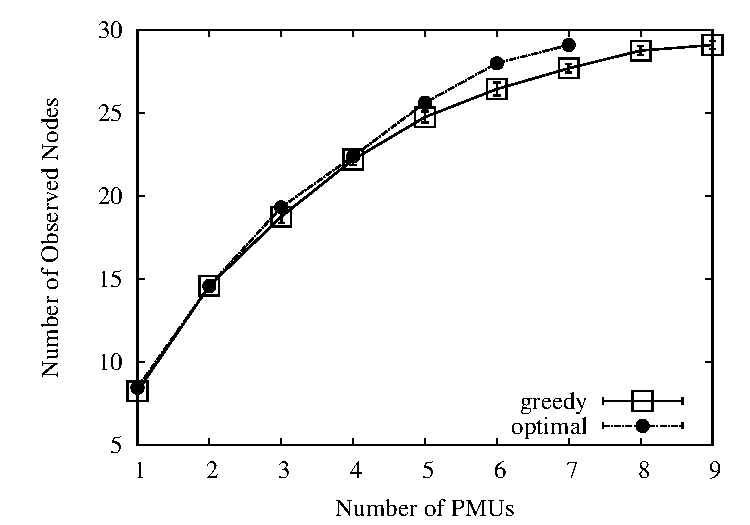
\includegraphics[scale=0.55]{figs/bus30.pdf}}
    \subfigure[Graphs based on IEEE Bus $57$]{\label{fig:bus57}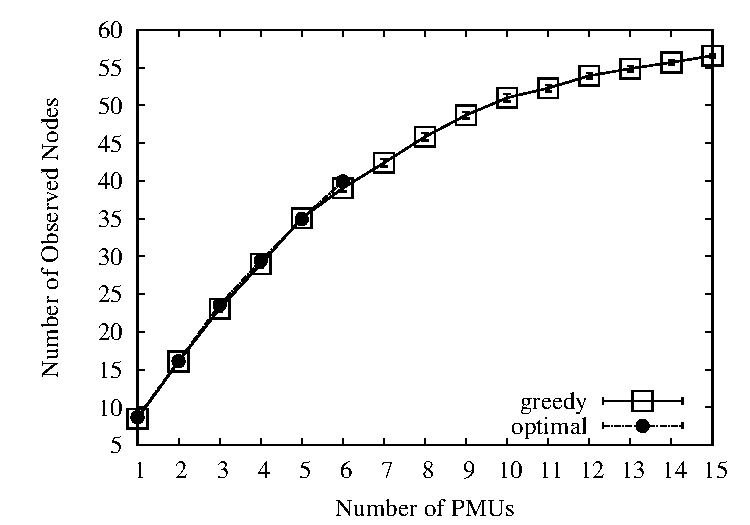
\includegraphics[scale=0.55]{figs/bus57.pdf}}
    \subfigure[Graphs based on IEEE Bus $118$]{\label{fig:bus118}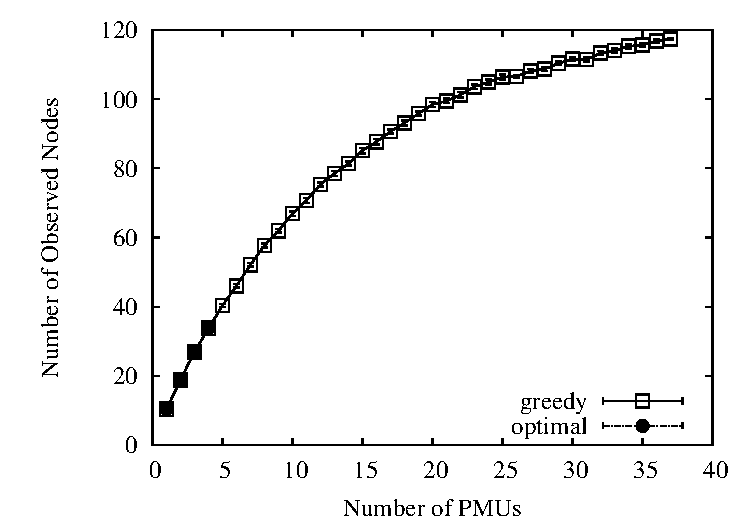
\includegraphics[scale=0.55]{figs/bus118.pdf}}
  \end{center}
	\caption{Mean number of observed nodes over synthetic graphs -- using {\tt greedy} and {\tt optimal} -- when varying number of PMUs. The $90\%$ confidence interval is shown.}
  \label{fig:maxinc-res}
\end{figure*}

\begin{figure*}[t]
  \begin{center}
    \subfigure[Graphs based on IEEE Bus $30$]{\label{fig:xvbus30}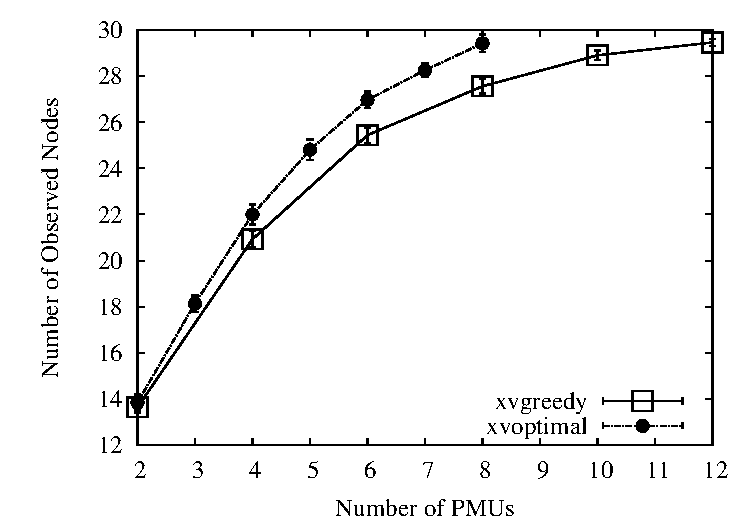
\includegraphics[scale=0.55]{figs/xvbus30.pdf}}
    \subfigure[Graphs based on IEEE Bus $57$]{\label{fig:xvbus57}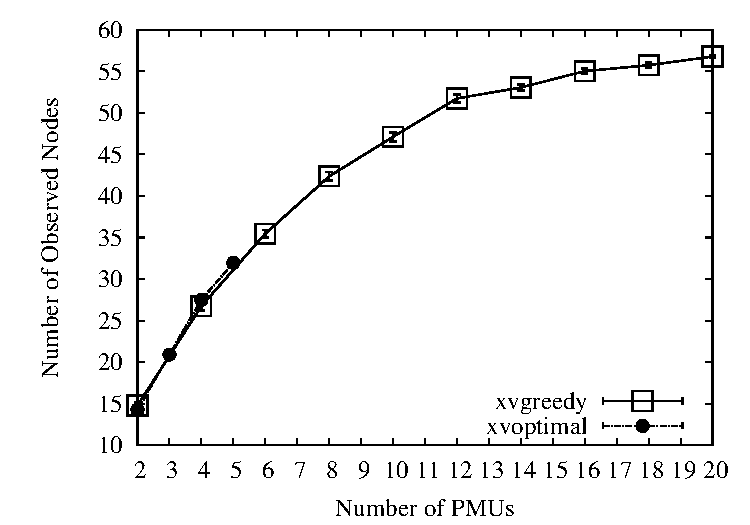
\includegraphics[scale=0.55]{figs/xvbus57.pdf}}
    \subfigure[Graphs based on IEEE Bus $118$]{\label{fig:xvbus118}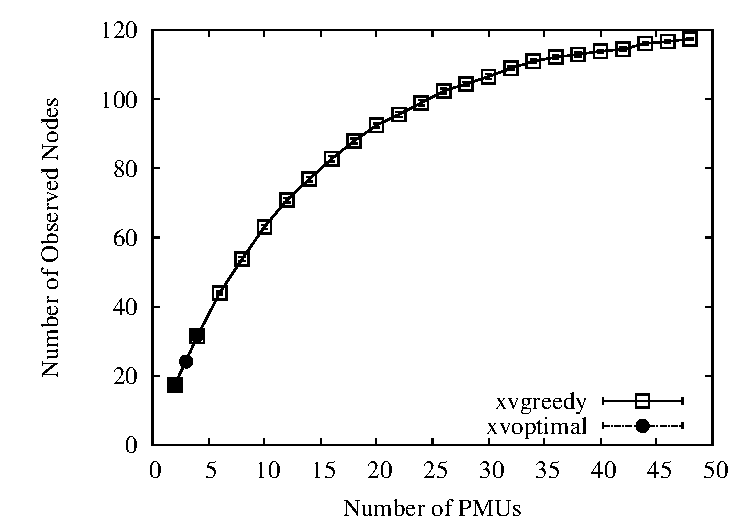
\includegraphics[scale=0.55]{figs/xvbus118.pdf}}
  \end{center}
	\caption{Over synthetic graphs, mean number of observed nodes -- using {\tt xvgreedy} and {\tt xvoptimal} -- when varying number of PMUs. The $90\%$ confidence interval is shown.}
  \label{fig:xv-res}
\end{figure*}




%\begin{figure}[t]
%\centering
%\includegraphics[scale=0.50]{figs/all118.pdf}
%\caption{Simulation results for \maxinc and \xvalpart using IEEE bus $118$.}
%\label{fig:all118}
%\end{figure}

\subsection{Simulation 2: Impact of Number of Zero-Injection Nodes}
\label{subsec:zero}

Next, we examine the impact of $|V_Z|$ on algorithm performance. 
For each synthetic graph, we run our algorithms for increasing values of $|V_Z|$ and determine the minimum number of PMUs needed to observe all nodes in the graph ($k^*$).
For each $z:=|V_Z|$, we select $z$ nodes uniformly at random to be zero-injection, and the rest are in $V_I$. Because we compute $k^*$ here, we solve \full and \xvals, rather than
\maxinc and \xvalparts as in Simulation 1.

We generate each data point using a similar procedure to the one described in Section \ref{subsec:synth}.  
For each $z=z_i$, we generate a graph and determine $k^*$. %the minimum number of PMUs needed to observe all nodes in the graph ($k^*$).  
We then compute $\overline{k^*}$, the mean value of $k^*$ over all simulation runs with $|V_Z| = z_i$.
We continue this procedure until $[0.9(\overline{k^*}),1.1(\overline{k^*})]$ falls within the $90\%$ confidence interval.

Figure \ref{fig:zero57} shows the simulation results for solving \full and \xval on synthetic graphs modeled by IEEE bus $57$. Results for other topologies considered here 
(i.e., $14$, $30$ and $118$) followed the same trend and are thus omitted. Due to the exponential running time of {\tt optimal} and {\tt xvoptimal}, we present here only results of our 
greedy algorithms. 

As expected, increasing the number of zero-injection nodes -- for both {\tt greedy} and {\tt xvgreedy} -- reduces the number of PMUs required for 
full observability. 
More zero-injection nodes allow O2 to be applied more frequently (Figure \ref{fig:o2}), thereby increasing the number of observed nodes without using more PMUs.
In fact, we found the relationship between $|V_Z|$ to the greedy estimate of $k^*$  to be linear.

The gap in $k^*$ between {\tt greedy} and {\tt xvgreedy} decreases as $z$ grows. {\tt greedy} and {\tt xvgreedy} observe a similar
number of nodes via O2 across all $z$ values: the mean absolute difference in the number of nodes observed by O2 between the two algorithms is $1.66$ nodes.  
Thus, as $z$ grows the number of nodes observed by O2 accounts for an increasing proportion of all observed nodes (Figure \ref{fig:o2}), causing the gap between {\tt greedy} and {\tt xvgreedy} to shrink.
%This statistic is confirmed visually by referring to Figure \ref{fig:o2} where the error bars (e.g., the $90\%$ confidence interval) for each data point are overlapping.  Thus, the number of nodes observed by O1 
%-- {\tt greedy} observes more nodes via O1 than {\tt xvgreedy} -- accounts for the difference between the two greedy algorithms. 
%We conclude that becuase the number of O2 observed nodes increases super-linearly with $z$ the gap between {\tt greedy} and {\tt xvgreedy} shrinks.


%\begin{figure*}[t]
%  \begin{center}
%    \subfigure[Graphs based on IEEE Bus $30$]{\label{fig:xvbus30}\includegraphics[scale=0.45]{figs/zero30.pdf}}
%    \subfigure[Graphs based on IEEE Bus $57$]{\label{fig:xvbus57}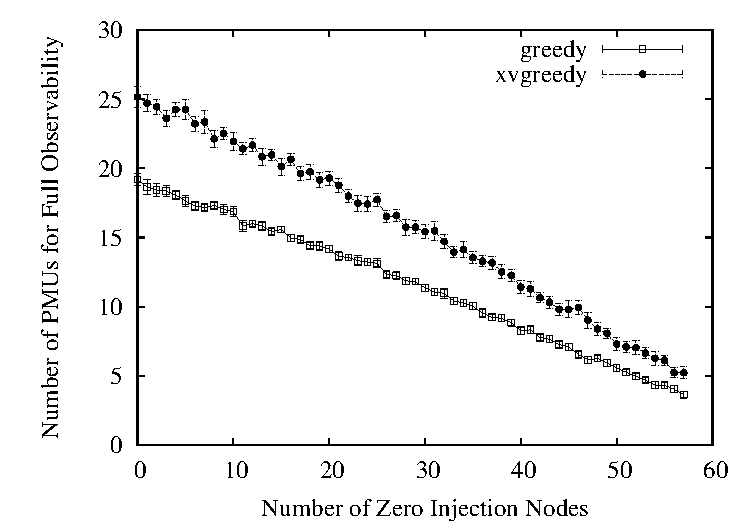
\includegraphics[scale=0.45]{figs/zero57.pdf}}
%    \subfigure[Graphs based on IEEE Bus $118$]{\label{fig:xvbus118}\includegraphics[scale=0.45]{figs/zero118.pdf}}
%  \end{center}
%	\caption{Simulation Results for \full and \xval greedy approximations, in which we vary the number of zero-injection nodes and determine the minimum number of PMUs needed to observe all nodes. 
%	{\tt xvgreedy} refers to the greedy algorithm with cross-validation and {\tt greedy} denotes the greedy algorithm without cross-validation. The $90\%$ confidence interval is shown. }
%  \label{fig:zero}
%\end{figure*}

\begin{figure*}[t]
  \begin{center}
    \subfigure[\underline{Simulation 2}: Number of PMUs needed for full observability for different $|V_Z|$ values, using synthetic graphs based on IEEE Bus $57$.]{\label{fig:zero57}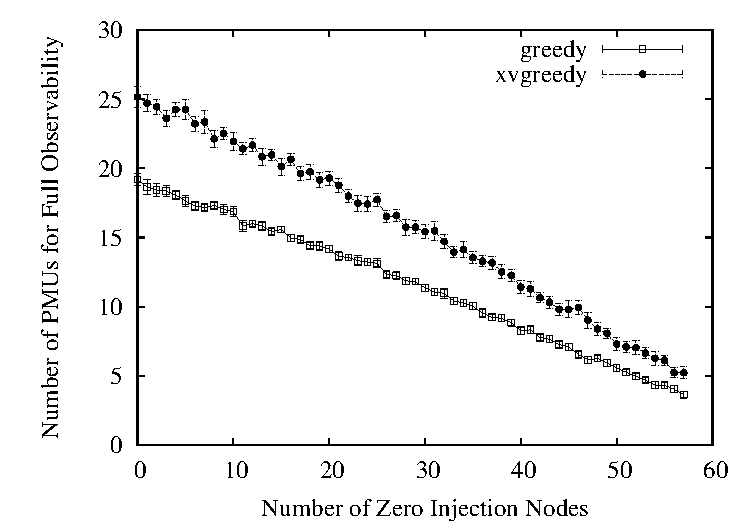
\includegraphics[scale=0.55]{figs/zero57.pdf}}
    \subfigure[\underline{Simulation 2}: Number of nodes observed by O2 for different $|V_Z|$ values, using synthetic graphs based on IEEE Bus $57$.] {\label{fig:o2}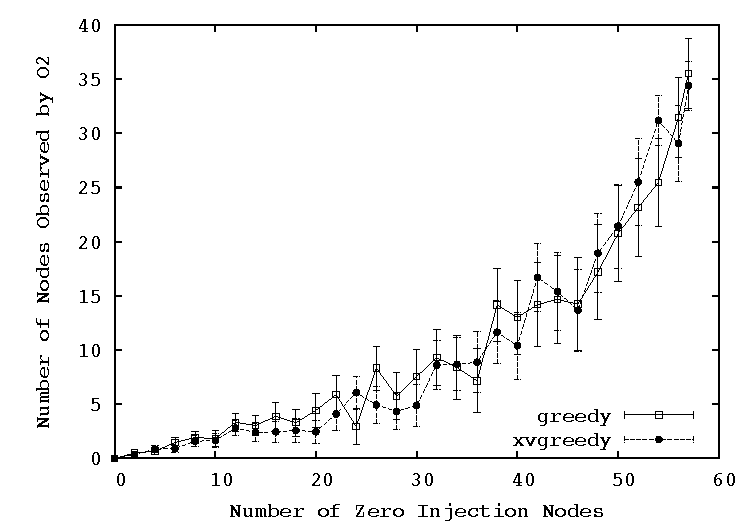
\includegraphics[scale=0.55]{figs/o2-b57.pdf}}
    \subfigure[\underline{Simulation 3}: Number of observed nodes when varying number of PMUS, using IEEE Bus $57$]{\label{fig:single57}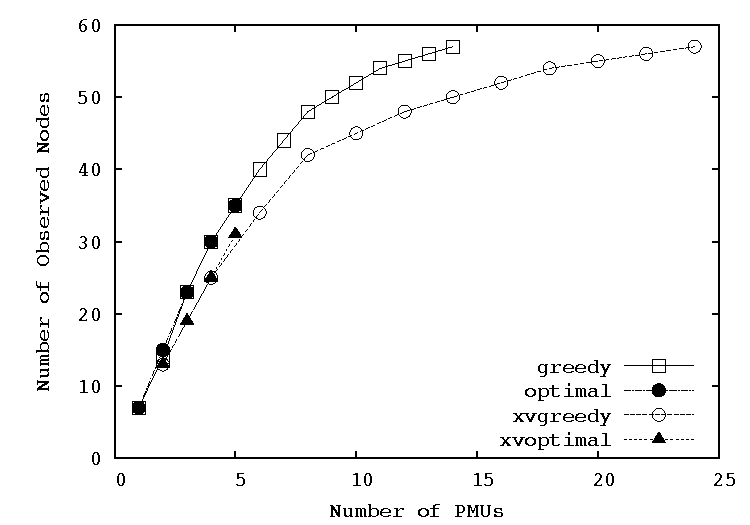
\includegraphics[scale=0.55]{figs/bus-single57.pdf}}
  \end{center}
	\caption{Results for Simulation 2 and 3. In Figures (a) and (b) the $90\%$ confidence interval is shown. }
  \label{fig:sim23}
\end{figure*}


\subsection{Simulation 3: Synthetic vs Actual IEEE Graphs}
\label{subsec:ieee}
In this section, we compare our results with the performance over the original IEEE systems. 
We assign nodes to $V_Z$ and $V_I$ as specified in the IEEE database files. Our results indicate that the trends we observed over the synthetic graphs apply as well to real topologies.


%When repeating Simulation 1, we find the same trends using the IEEE topologies. %as with the synthetic graphs.
Figure \ref{fig:single57} shows the number of observed nodes for the {\tt greedy},  {\tt xvgreedy}, {\tt optimal},  and {\tt xvoptimal} algorithms %when we vary the number of PMUs
for IEEE bus system $57$. {\tt greedy} and {\tt xvgreedy} observe nearly as many nodes as the corresponding optimal solution.
%For both with and without cross-validation, the greedy algorithm observes nearly as many nodes as the {\tt optimal} solution.
In many cases, greedy yields the optimal placement. %These results are consistent with our findings for IEEE bus system $14$, $30$, and $118$.
%Similarly, when repeating Simulation 2 using the actual IEEE bus systems, we observe the same trends described in Section \ref{subsec:zero}.
Similarly, as with the synthetic graphs, the number of PMUs required to observe all nodes decreases linearly as $|V_Z|$ increases.
{\footnote {\small The same trends were observed using IEEE bus systems $14$, $30$, and $118$.}}

\begin{table}
\begin{center}
\begin{tabular}{|l|l|l|l|l|}
\hline
 &  {\tt greedy} & {\tt xvgreedy}  & {\tt optimal} & {\tt xvoptimal}  \\
\hline \hline
Simulation 1  & $4\%$  & $4.6\%$ & $6\%$ & $7.6\%$  \\
\hline
Simulation 2 & $9.1\%$ & $16.1\%$ & N/A  & N/A  \\
\hline
\end{tabular}
\end{center}
\caption{Mean absolute difference between the computed values from synthetic graphs and IEEE graphs, normalized by the result for the synthetic graph.}
%\caption{Mean absolute difference between the computed values of each synthetic graph data point and corresponding IEEE graph data point.}
\label{tab:diff}
\end{table}

To compare the actual values for synthetic graphs to those over IEEE graphs, we took the mean absolute difference between the results, and normalized by the result for the synthetic graph.
%For example, let $n_{G',k}$ be the output of {\tt greedy} for solving \maxinc for synthetic graph $G'$ and $k$, and let $n_{G,k}$ be the same for the corresponding IEEE graph.
For example, let $n_{k}$ be the mean number of observed nodes using {\tt greedy} over all synthetic graphs with input $k$, and let $n_{G,k}$ 
be the output of {\tt greedy} for IEEE graph $G$ and $k$.
We compute $n_{d,k}=(|n_{k}-n_{G,k}|)/n_{k}$.  Finally, we calculate the mean over all $n_{d,k}$.
This process is done for each algorithm we evaluate.
The resulting statistics can be found in Table \ref{tab:diff}.  The small average difference between the synthetic graphs and the
actual IEEE topologies suggests that the node degree distribution of the IEEE graph is an effective feature for generating similar synthetic graphs.
%{\footnote {\small The average difference is larger for Simulation 2 because the $k^*$ value is sensitive to the assignment of zero-injection nodes.  Recall that the zero
%injection nodes are assigned uniformely at random and for the IEEE topology we only have a single  SHOULD AVG OVER MANY ZERO INJECTION NODE ASSIGNMENTS}}
